\documentclass[10pt,a4paper]{article}
\usepackage[utf8]{inputenc}
\usepackage{amsmath}
\usepackage{amsfonts}
\usepackage{amssymb}
\usepackage{graphicx}
\usepackage{subcaption}
\begin{document}
	\title{\texttt{RprobitB} application to \texttt{Train} dataset}
	\author{Lennart Oelschläger}
	\date{\today}
	\maketitle
	The \texttt{Train} dataset from the R-package \texttt{mlogit} constitutes a
	\begin{itemize}
		\item stated preference survey in Netherlands,
		\item each individual ($N = 235$) responding to several scenarios ($T = 5\dots19$),
		\item where for every scenario, two train trips ($J = 2$) are proposed 
		\item with different combinations of 4 attributes: \texttt{price}, \texttt{travel time}, \texttt{number of changes} and the \texttt{class of comfort}.
	\end{itemize}
	We z-standardize the covariates.
	The \texttt{cost} attribute is fixed to the value -1. The \texttt{class of comfort} attribute is connected to a fixed coefficient.
	\begin{table}[h]
		\centering
		\begin{tabular}{c|c|c|c|l}
			Model & $C$ & $C$ update & fixed coefficients & random coefficients \\ \hline
			1	  &  1  &  no  &  & \texttt{travel time}, \texttt{number of changes} \\ \hline
			2  	  &  2  &  no  &  & \texttt{travel time}, \texttt{number of changes} \\ \hline
			3	  &  3  &  no  &  & \texttt{travel time}, \texttt{number of changes} \\ \hline
			4	  &  2  &  yes &  & \texttt{travel time}, \texttt{number of changes} \\ \hline
			5     &  1  &  no  & \texttt{number of changes} & \texttt{travel time} \\ \hline
			6     &  2  &  no  & \texttt{number of changes} & \texttt{travel time} \\ \hline
			7     &  2  &  yes & \texttt{number of changes} & \texttt{travel time} \\ 
		\end{tabular}
		\caption{Model definitions}
	\end{table}
	\begin{table}[h]
		\centering
		\begin{tabular}{c|r|r|r}
			Model & WAIC & dWAIC & Akaike weight \\ \hline
			1 & 4897.034 & 0.0000 	 & 0.9886 \\ \hline
			5 & 4905.953 & 8.9189    & 0.0114 \\ \hline
			6 & 6488.273 & 1591.2387 & 0.0000 \\ \hline
			7 & 6557.075 & 1660.0407 & 0.0000 \\ \hline
			2 & 6609.486 & 1712.4519 & 0.0000 \\ \hline
			4 & 6822.989 & 1925.9545 & 0.0000 \\ \hline
			3 & 7882.325 & 2985.2909 & 0.0000 \\ 
		\end{tabular}
		\caption{Model comparison (best to worst)}
	\end{table}
	\begin{figure*}[h!]
		\centering
		\begin{subfigure}[t]{0.5\textwidth}
			\centering
				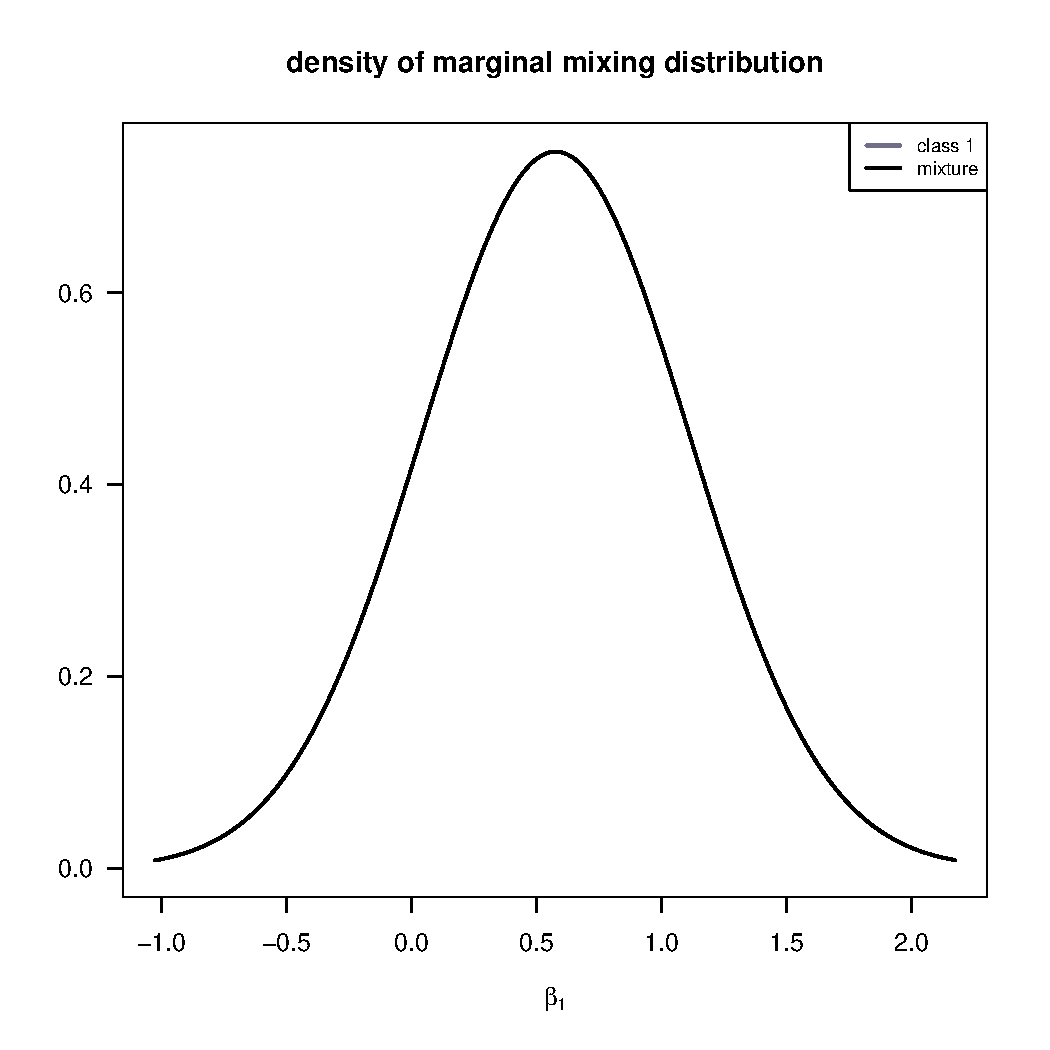
\includegraphics[width=5cm]{results/train_C1/marginal.pdf}
			\caption{Mixing distribution}
		\end{subfigure}%
		~ 
		\begin{subfigure}[t]{0.5\textwidth}
			\centering
				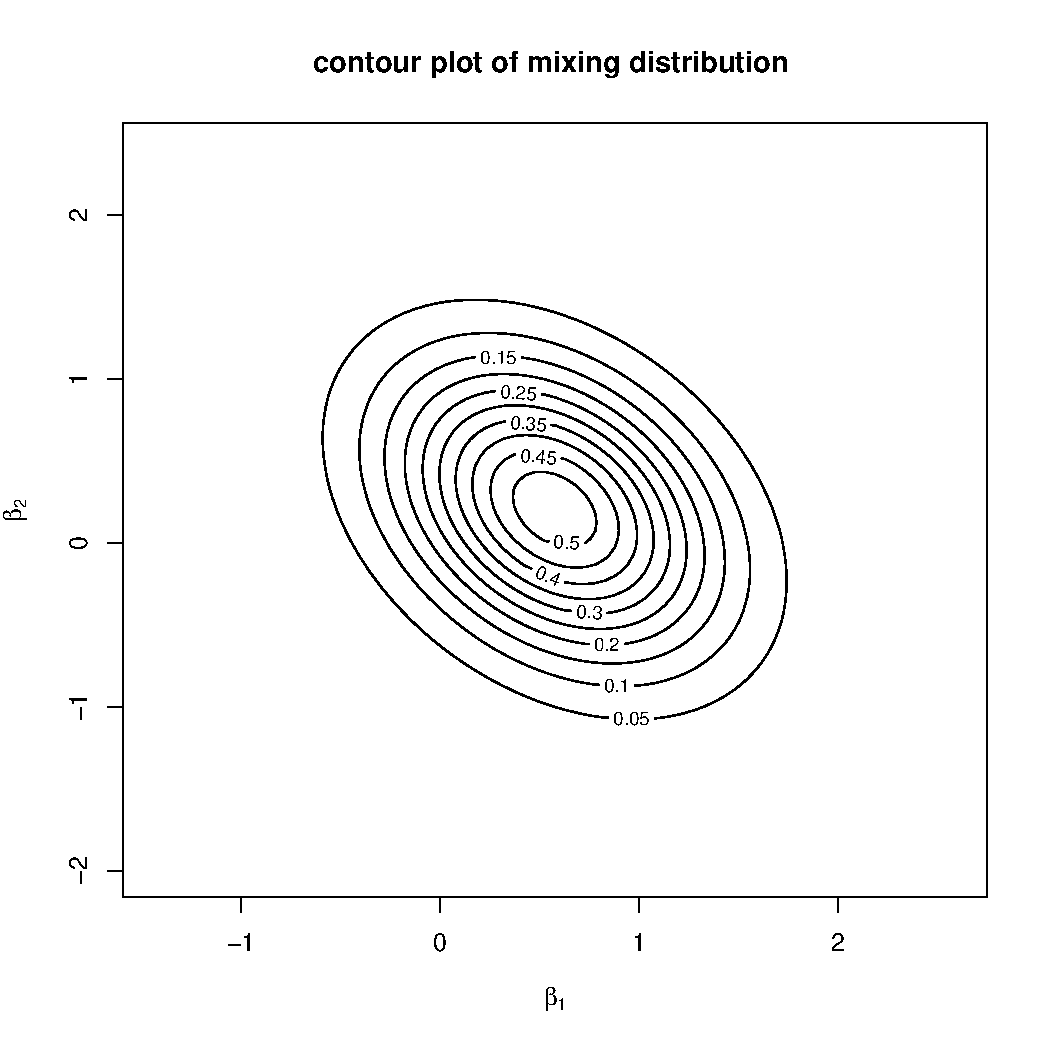
\includegraphics[width=5cm]{results/train_C1/contour.pdf}
			\caption{Contour plot}
		\end{subfigure}
		\caption{Model 1}
	\end{figure*}
	\begin{figure*}[h!]
		\centering
		\begin{subfigure}[t]{0.5\textwidth}
			\centering
			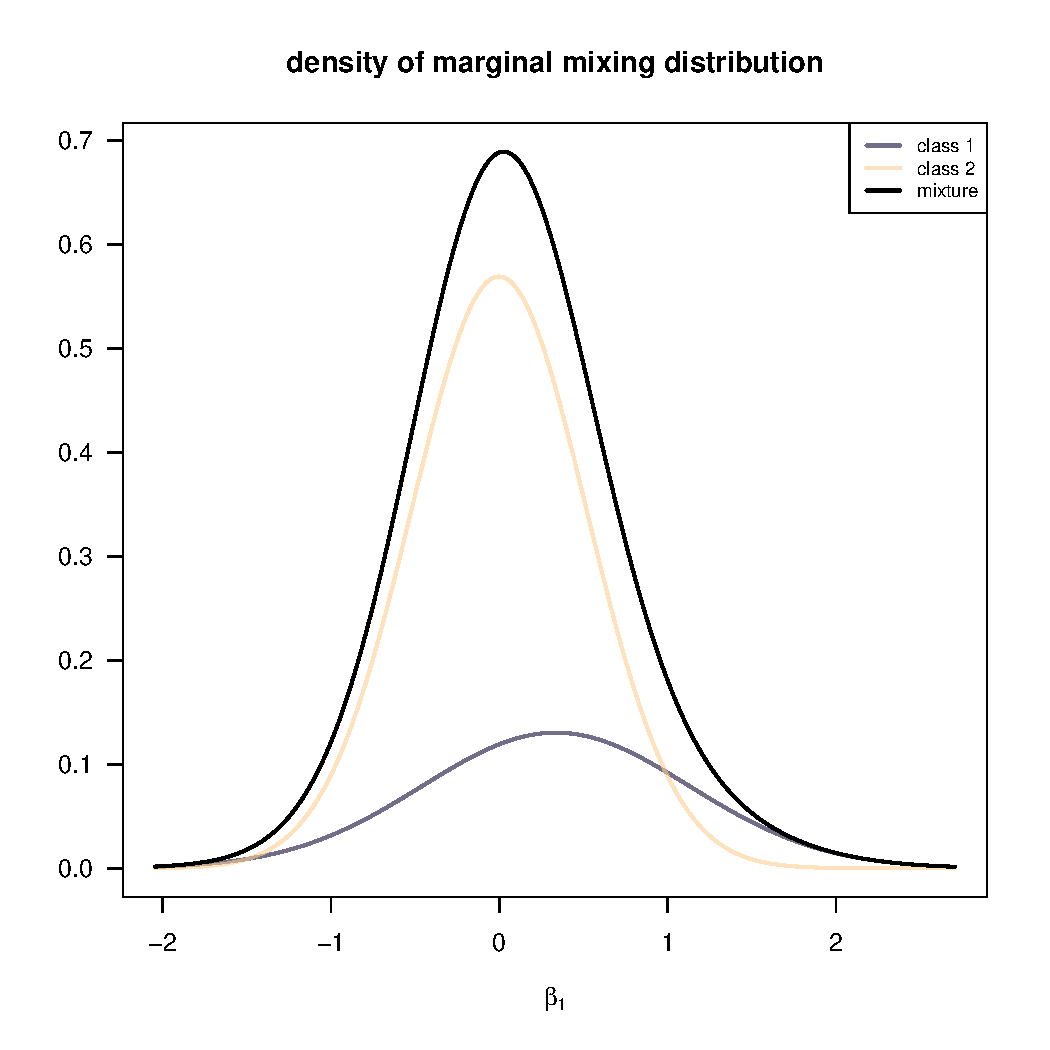
\includegraphics[width=5cm]{results/train_C2/marginal.pdf}
			\caption{Mixing distribution}
		\end{subfigure}%
		~ 
		\begin{subfigure}[t]{0.5\textwidth}
			\centering
			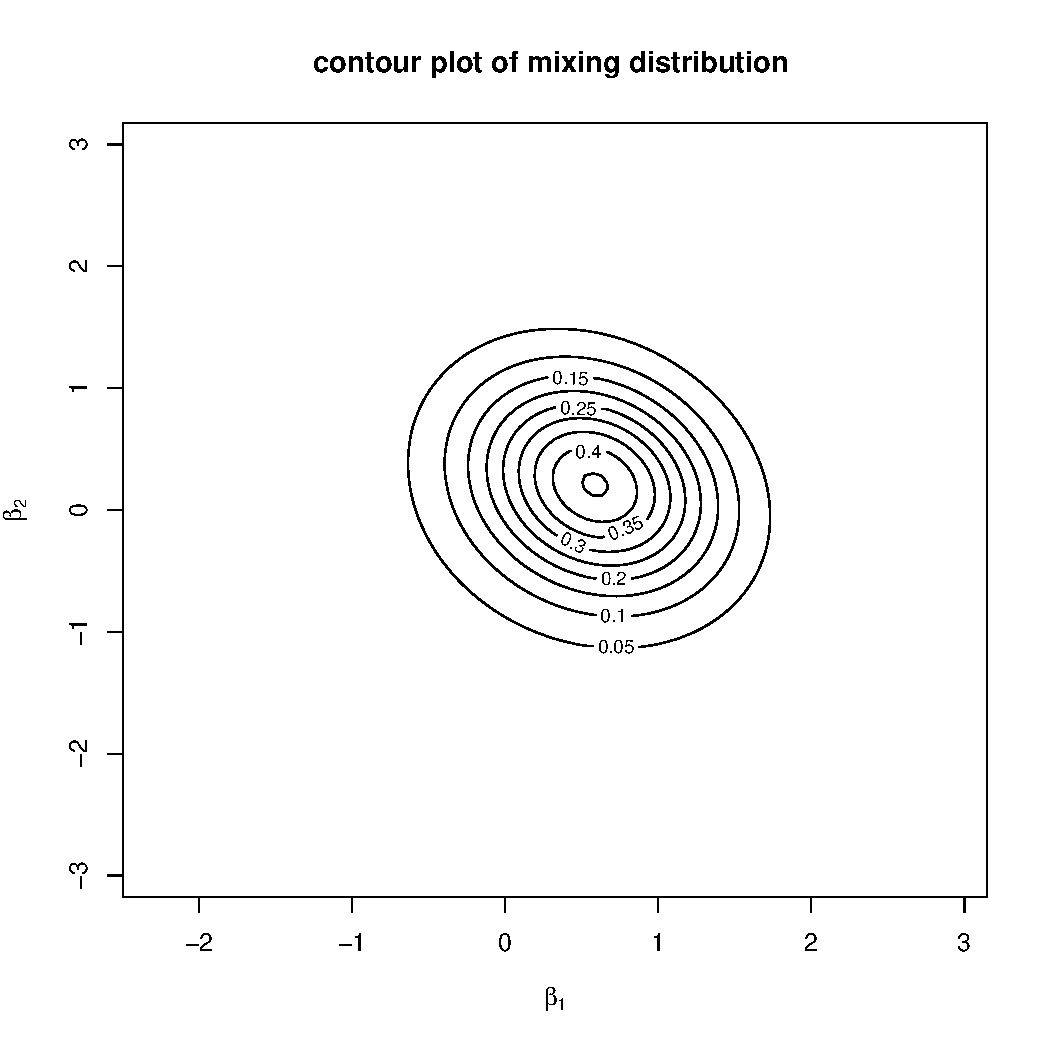
\includegraphics[width=5cm]{results/train_C2/contour.pdf}
			\caption{Contour plot}
		\end{subfigure}
		\caption{Model 2}
	\end{figure*}
	\begin{figure*}[h!]
		\centering
		\begin{subfigure}[t]{0.5\textwidth}
			\centering
			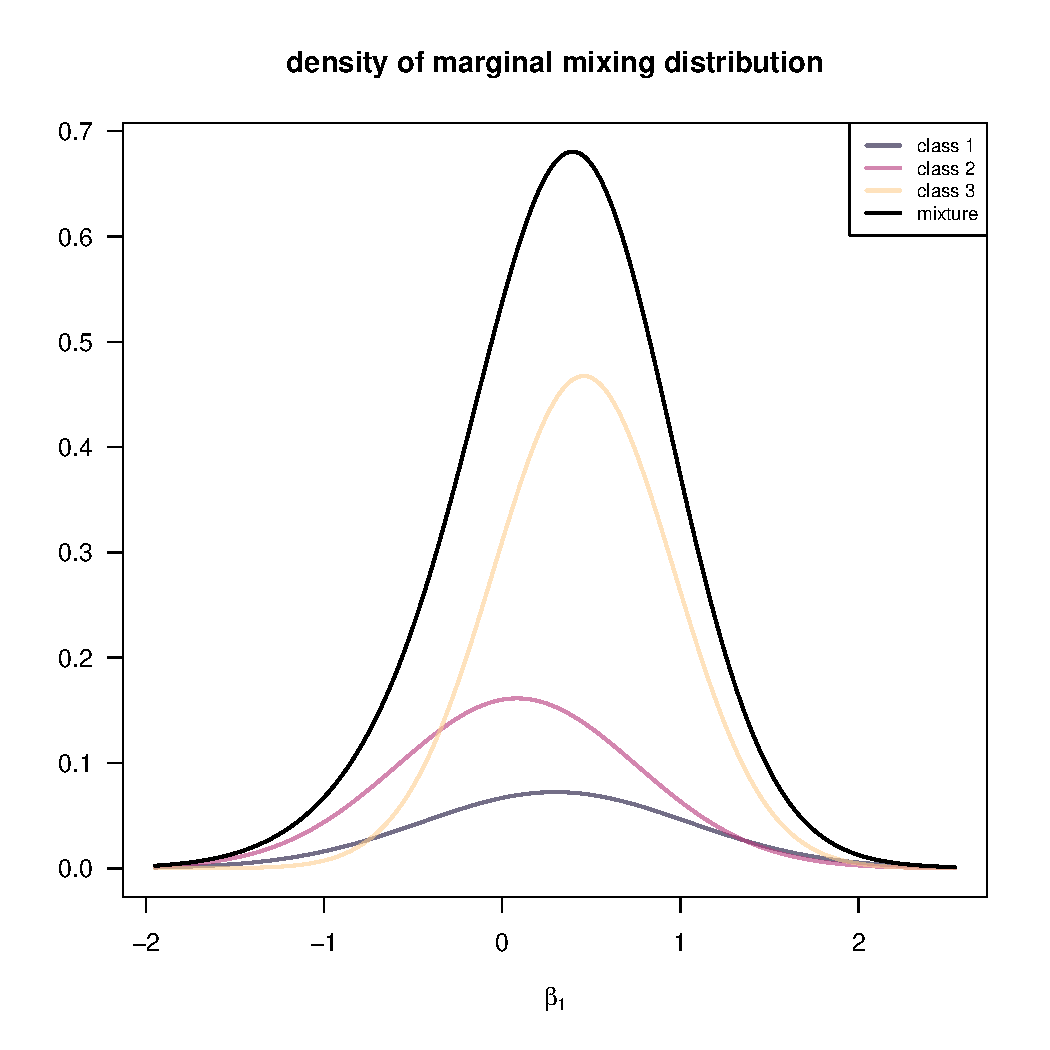
\includegraphics[width=5cm]{results/train_C3/marginal.pdf}
			\caption{Mixing distribution}
		\end{subfigure}%
		~ 
		\begin{subfigure}[t]{0.5\textwidth}
			\centering
			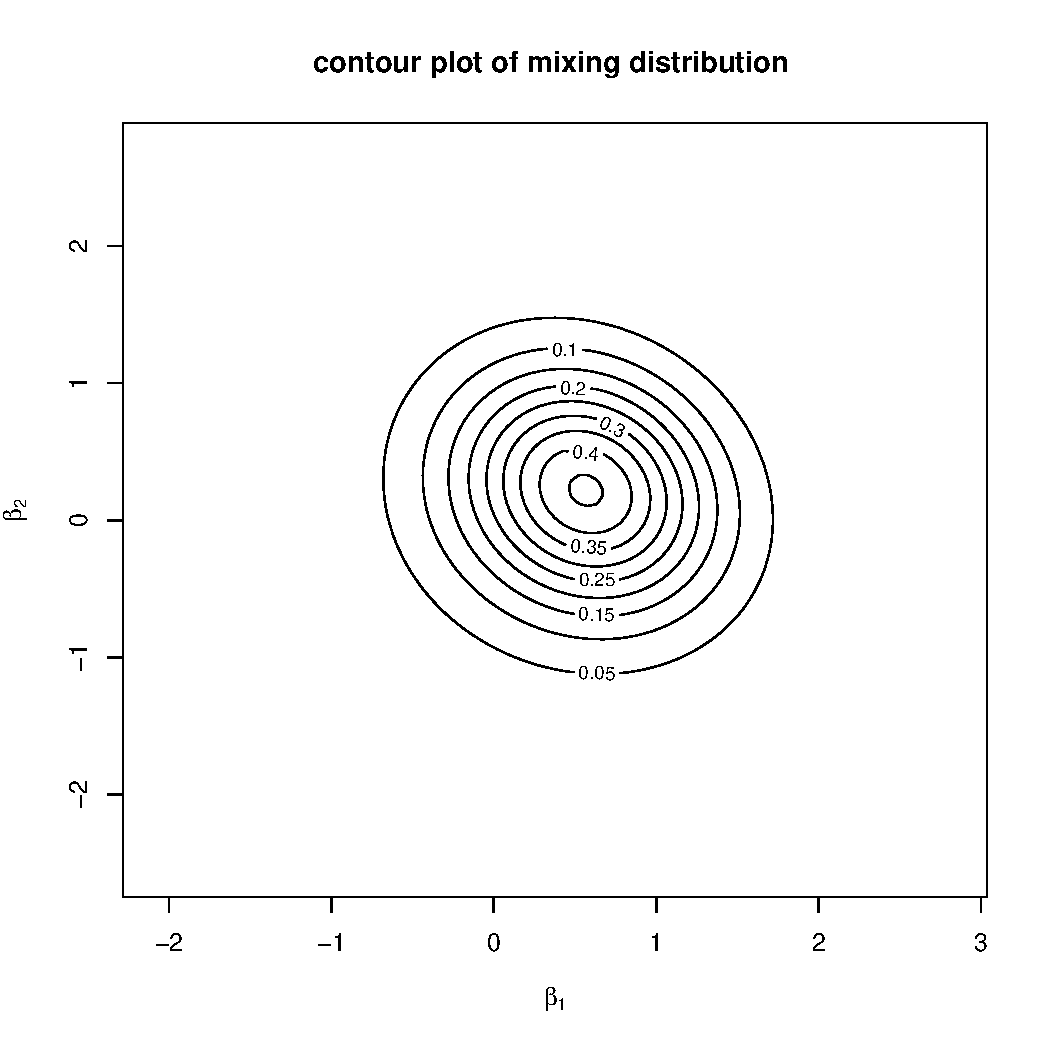
\includegraphics[width=5cm]{results/train_C3/contour.pdf}
			\caption{Contour plot}
		\end{subfigure}
		\caption{Model 3}
	\end{figure*}
	\begin{figure*}[h!]
		\centering
		\begin{subfigure}[t]{0.5\textwidth}
			\centering
			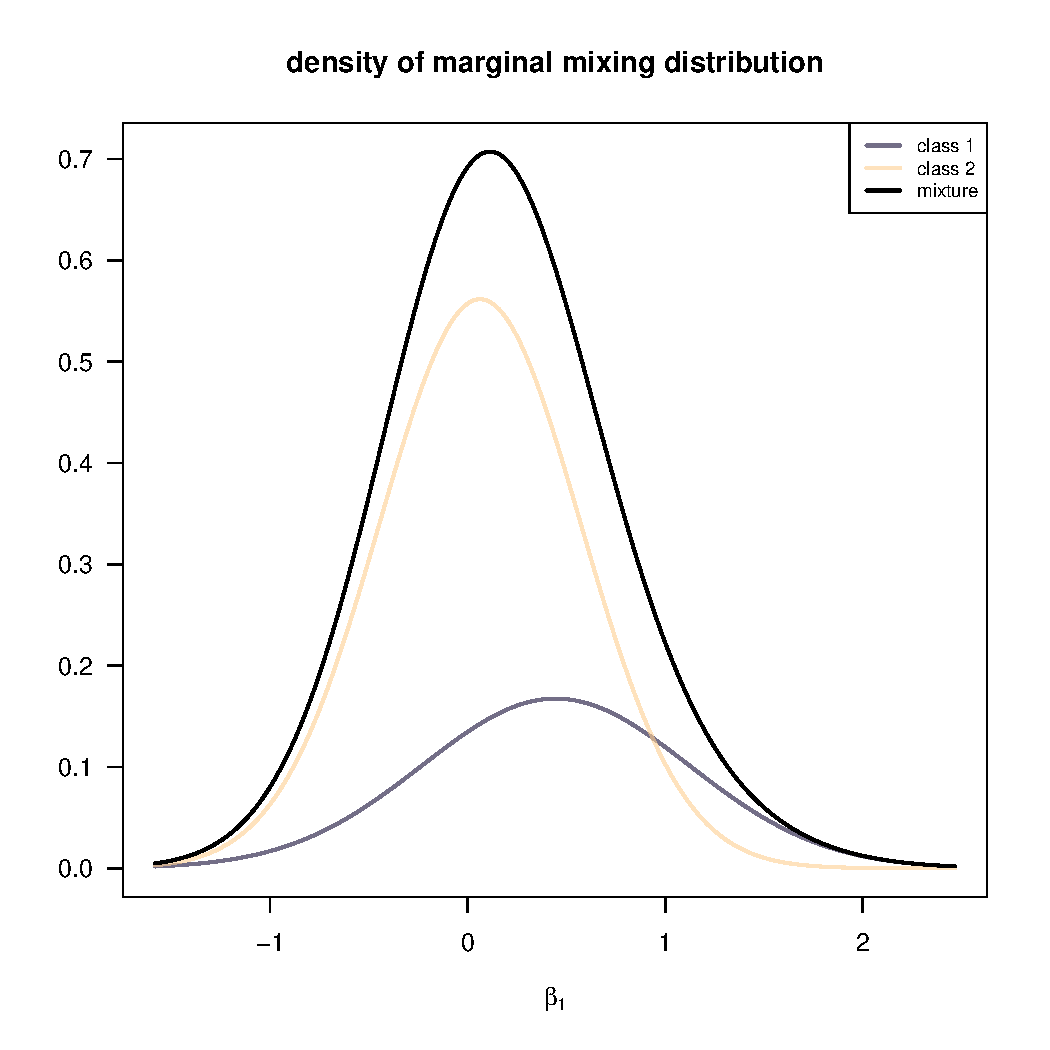
\includegraphics[width=5cm]{results/train_Cf/marginal.pdf}
			\caption{Mixing distribution}
		\end{subfigure}%
		~ 
		\begin{subfigure}[t]{0.5\textwidth}
			\centering
			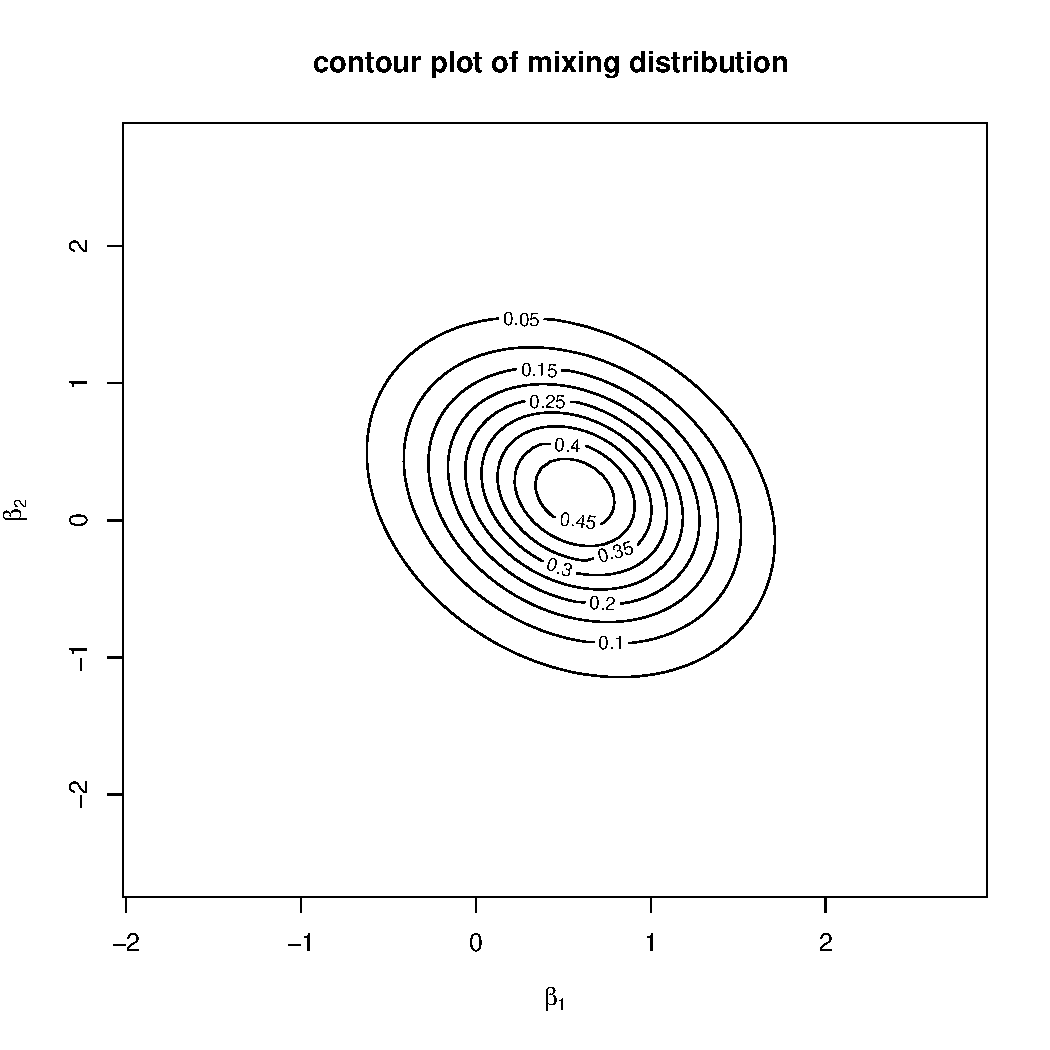
\includegraphics[width=5cm]{results/train_Cf/contour.pdf}
			\caption{Contour plot}
		\end{subfigure}
		\caption{Model 4}
	\end{figure*}
	\begin{figure*}[h!]
		\centering
		\begin{subfigure}[t]{0.3\textwidth}
			\centering
			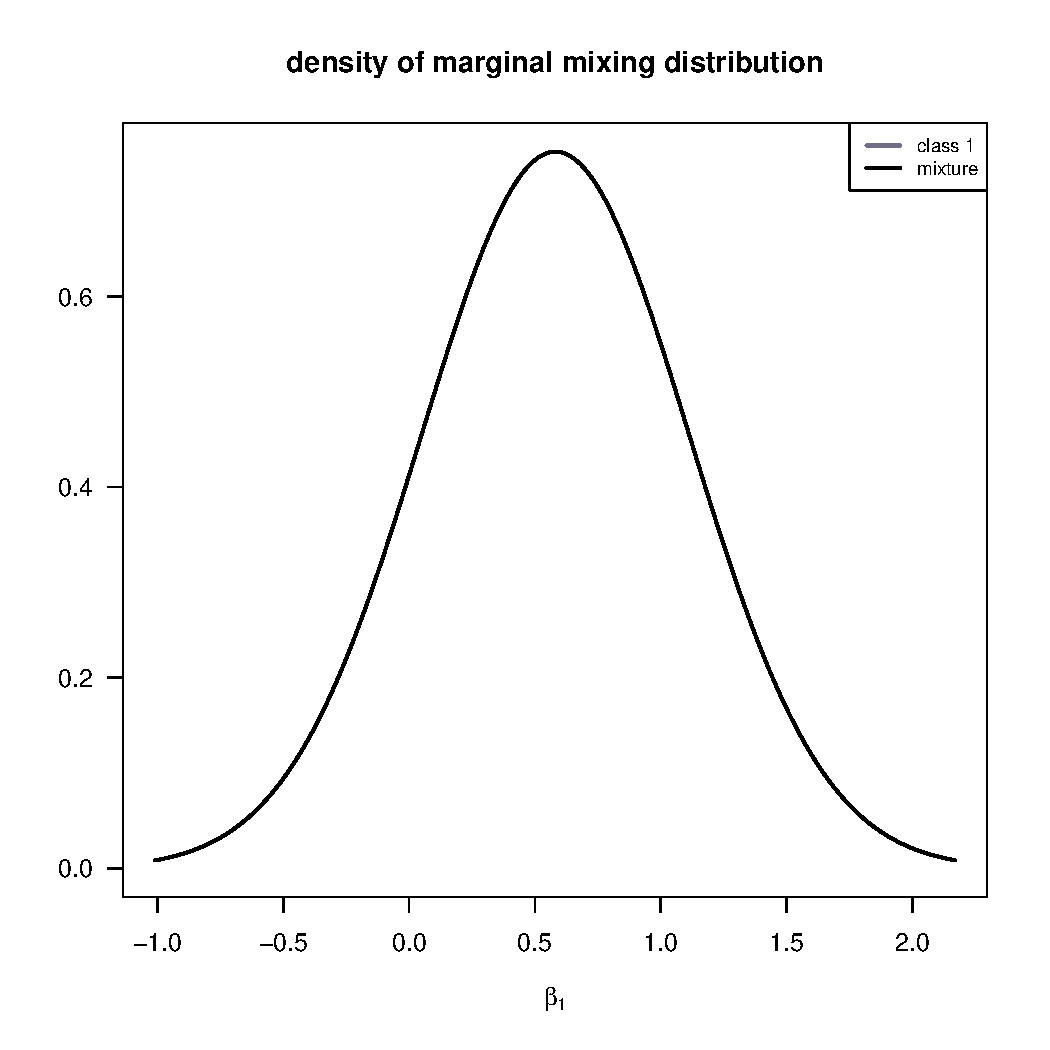
\includegraphics[width=4cm]{results/train_random_time_C1/marginal.pdf}
			\caption{Mixing distribution}
		\end{subfigure}%
		~ 
		\begin{subfigure}[t]{0.3\textwidth}
			\centering
			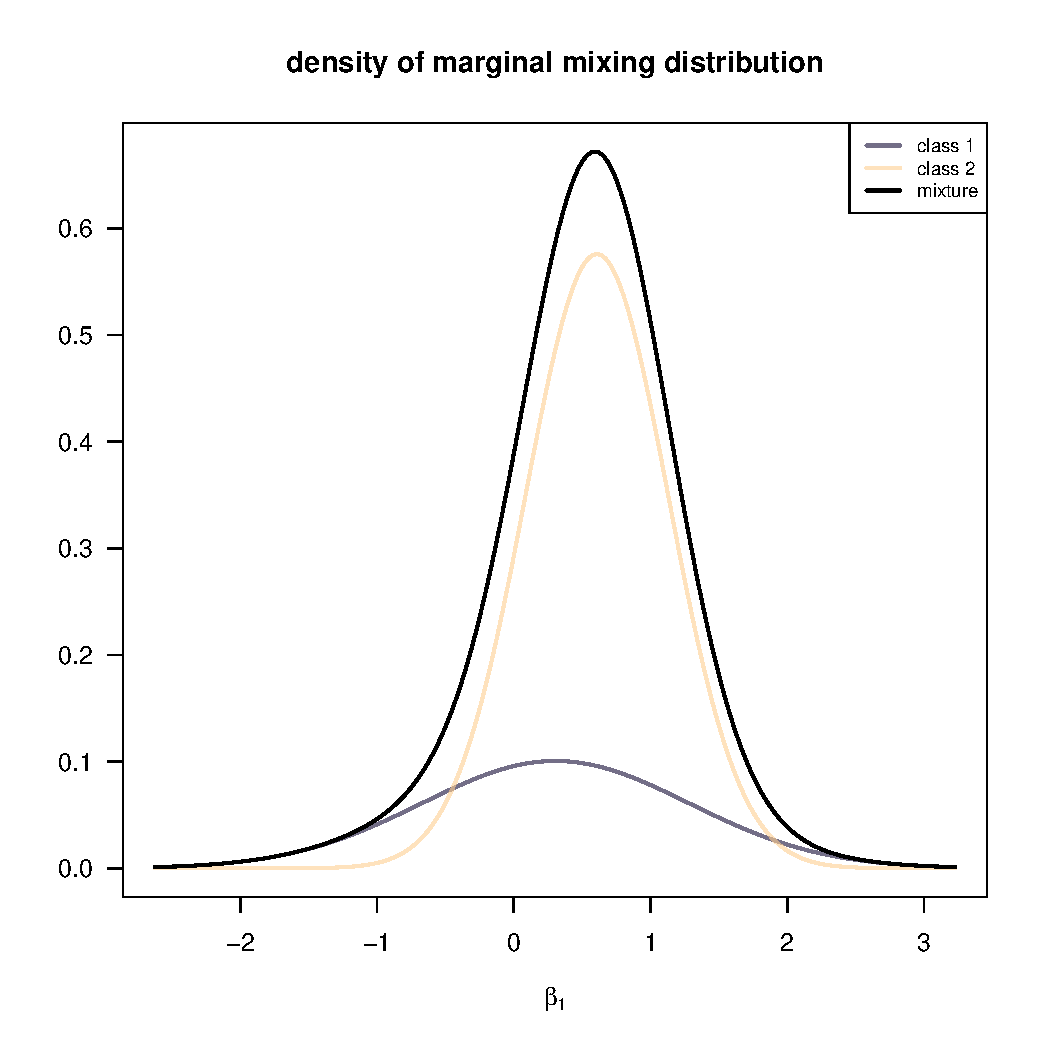
\includegraphics[width=4cm]{results/train_random_time_C2/marginal.pdf}
			\caption{Mixing distribution}
		\end{subfigure}
		~ 
		\begin{subfigure}[t]{0.3\textwidth}
			\centering
			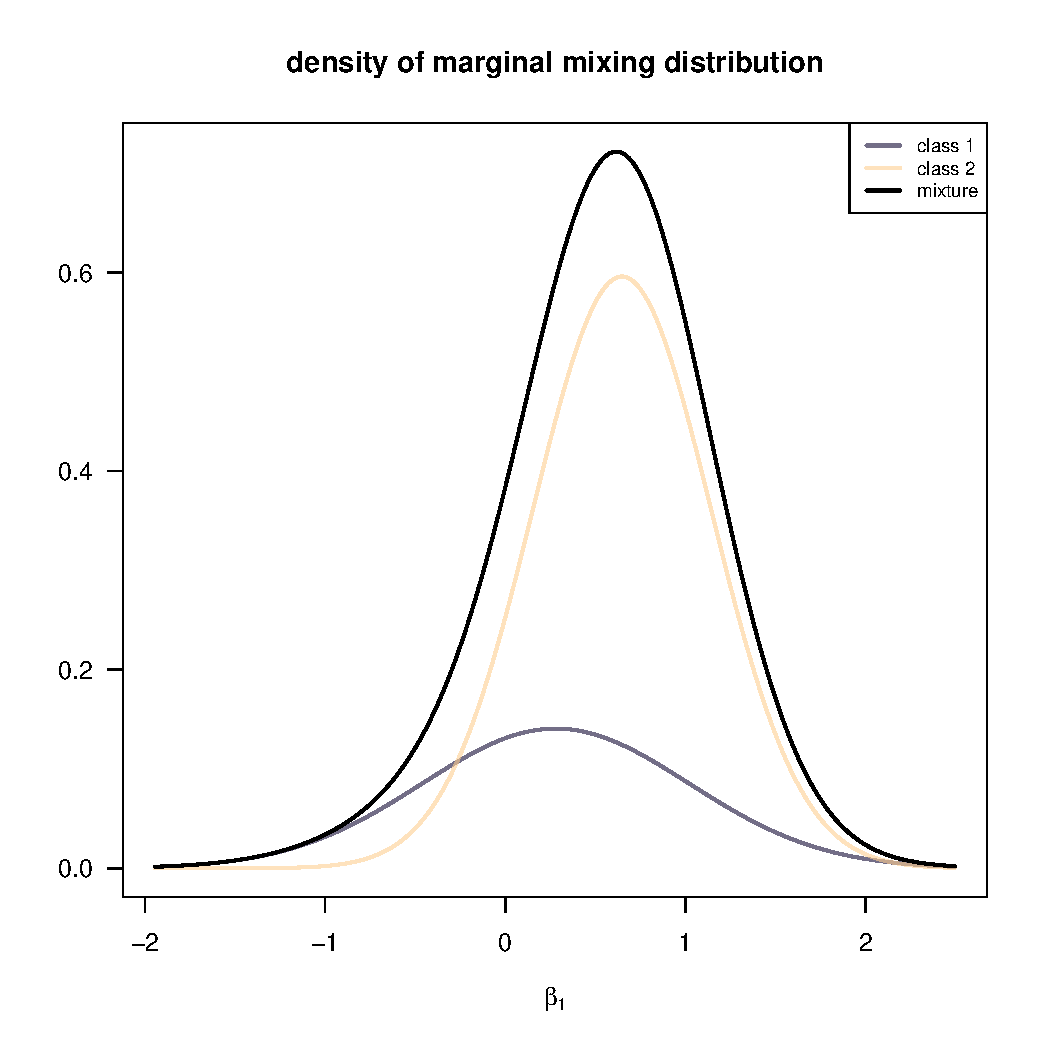
\includegraphics[width=4cm]{results/train_random_time_Cf/marginal.pdf}
			\caption{Mixing distribution}
		\end{subfigure}
		\caption{Model 5 - 7}
	\end{figure*}
\end{document}